\documentclass[]{article}
\usepackage{lmodern}
\usepackage{amssymb,amsmath}
\usepackage{ifxetex,ifluatex}
\usepackage{fixltx2e} % provides \textsubscript
\ifnum 0\ifxetex 1\fi\ifluatex 1\fi=0 % if pdftex
  \usepackage[T1]{fontenc}
  \usepackage[utf8]{inputenc}
\else % if luatex or xelatex
  \ifxetex
    \usepackage{mathspec}
  \else
    \usepackage{fontspec}
  \fi
  \defaultfontfeatures{Ligatures=TeX,Scale=MatchLowercase}
\fi
% use upquote if available, for straight quotes in verbatim environments
\IfFileExists{upquote.sty}{\usepackage{upquote}}{}
% use microtype if available
\IfFileExists{microtype.sty}{%
\usepackage[]{microtype}
\UseMicrotypeSet[protrusion]{basicmath} % disable protrusion for tt fonts
}{}
\PassOptionsToPackage{hyphens}{url} % url is loaded by hyperref
\usepackage[unicode=true]{hyperref}
\hypersetup{
            pdfborder={0 0 0},
            breaklinks=true}
\urlstyle{same}  % don't use monospace font for urls
\usepackage{graphicx,grffile}
\makeatletter
\def\maxwidth{\ifdim\Gin@nat@width>\linewidth\linewidth\else\Gin@nat@width\fi}
\def\maxheight{\ifdim\Gin@nat@height>\textheight\textheight\else\Gin@nat@height\fi}
\makeatother
% Scale images if necessary, so that they will not overflow the page
% margins by default, and it is still possible to overwrite the defaults
% using explicit options in \includegraphics[width, height, ...]{}
\setkeys{Gin}{width=\maxwidth,height=\maxheight,keepaspectratio}
\IfFileExists{parskip.sty}{%
\usepackage{parskip}
}{% else
\setlength{\parindent}{0pt}
\setlength{\parskip}{6pt plus 2pt minus 1pt}
}
\setlength{\emergencystretch}{3em}  % prevent overfull lines
\providecommand{\tightlist}{%
  \setlength{\itemsep}{0pt}\setlength{\parskip}{0pt}}
\setcounter{secnumdepth}{0}
% Redefines (sub)paragraphs to behave more like sections
\ifx\paragraph\undefined\else
\let\oldparagraph\paragraph
\renewcommand{\paragraph}[1]{\oldparagraph{#1}\mbox{}}
\fi
\ifx\subparagraph\undefined\else
\let\oldsubparagraph\subparagraph
\renewcommand{\subparagraph}[1]{\oldsubparagraph{#1}\mbox{}}
\fi

% set default figure placement to htbp
\makeatletter
\def\fps@figure{htbp}
\makeatother


\date{}

\begin{document}

\subsection{CSE 152 HW1}\label{cse-152-hw1}

Name: Zhouhang Shao PID: A99086018 \#\#\#Problem 1: Play with Colors
\#\#\#\#Question: Using your new found Matlab or Python skills, write a
program that does the following:

• Read in a color image.

• Resize the image to 256 x 256 pixels using bilinear interpolation.

• Tile the image to form 4 quadrants where

-- The top left quadrant is the original image

-- The top right is the green channel of the original image (other
channels set to zero)

-- The bottom left is the red channel (other channels set to zero)

-- The bottom right is the blue channel (other channels set to zero)
Test your program with the given image cleese.JPG. Expected output for
this task is given in Figure

\begin{enumerate}
\def\labelenumi{\arabic{enumi}.}
\tightlist
\item
  Then, write a short paragraph explaining your results. Does your
  program produce the correct output?
\end{enumerate}

\paragraph{My answer:}\label{my-answer}

Yes, my program produce the correct output. First, I initialized a 512 *
512 image(result\_image) and set all it's pixel value(all three
channels) to zero. Then, I used the imread() to read the `cleese.jpg',
resize it to size 256 * 256 using imresize() and put it at the top left
corner in my result\_image. The next step is to extract the different
channels of the the image that I previously read. I put the red channels
on the top right corner while put the green channel at the bottom left.
Finally, I put the blue channel at the bottom right.

The output is image is attached bellow:

\begin{figure}
\centering
\includegraphics{media/14916935985623/modified_cleese_1.png}
\caption{modified\_cleese\_1 -c}
\end{figure}

\paragraph{Source Code:}\label{source-code}

\begin{verbatim}
result_image = uint8(zeros(512,512,3));

%read and resize the image
I = imread('cleese.JPG');
%resize the image with bilinear interpolation to size 256 * 256
resize_image = imresize(I, [256,256],'bilinear');

%concatenating the resized image to the result image
result_image(1:256,1:256,:)=resize_image;
result_image(257:512,1:256,1)=resize_image(:,:,1); %Red

result_image(1:256,257:512,2)=resize_image(:,:,2); %Green

result_image(257:512,257:512,3)=resize_image(:,:,3); %Blue

figure,imshow(result_image);
imwrite(result_image,'modified_cleese.png') %write an output image
\end{verbatim}

\subsubsection{Problem 2: Image
Rotation}\label{problem-2-image-rotation}

\paragraph{Question:}\label{question}

Consider an image I. Write a function to rotate the I by θ radians
anticlockwise, θ ∈ \{0, π 2 , π, 3π 2 \}. Your function need not handle
other angles. Do NOT use built-in functions such as imrotate in MATLAB /
warpAffine in Python (OpenCV), or any other library function to rotate I.
Include four images in the report: I and three rotated images like in
Fig 2. You should run your function on the ucsd logo.png image provided
on the website and provide results only for that. \#\#\#\# My answer: My
rotation function takes an source image and rotational angle(in radian)
as inputs and output a rotated image . The function will map the pixel
of the result image from the corresponding pixel in the input image. The
mapping is slightly different depends on the rotation angles. All the
source code and resulting images are attached at the end.

\paragraph{Source code}\label{source-code-1}

\begin{verbatim}
function [result] = rotate_img(src, r)
    dim = size(src);
    h = dim(1);
    w = dim(2); 
    
    if r == pi/2    %rotating 90 degrees
        for i = 1 : 3
            for x = 1 : h
                for y = 1 : w
                    result(w-y+1,x,i) = src(x,y,i);
                end
            end
        end
    elseif r == pi  %rotating 180 degrees
        for i = 1 : 3
            for x = 1 : h
                for y = 1 : w  
                    result(h-x+1,w-y+1,i)=src(x,y,i);
                end
            end
        end
    elseif r == (pi*3)/2  %rotating 180 degrees
        for i = 1 : 3
            for x = 1 : h
                for y = 1 : w
                    result(y, h - x + 1,i) = src(x,y,i);
                end
            end
        end
    else %default case: the image remains the same
        for i = 1 : 3
            for x = 1 : h
                for y = 1 : w
                    result(x,y,i) = src(x,y,i); %make a copy of source img
                end
            end
        end
    end
end
\end{verbatim}

\begin{itemize}
\tightlist
\item
  Rotating 0 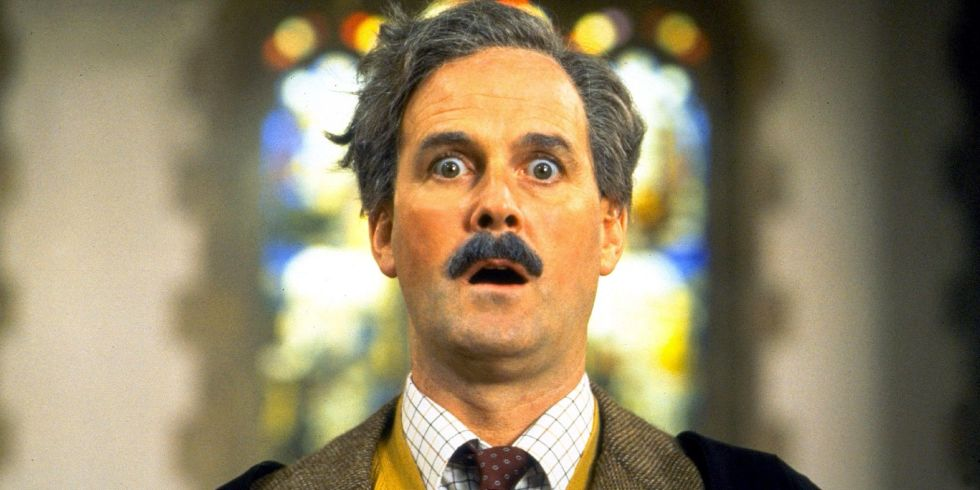
\includegraphics{media/14916935985623/rotated0.png}
\item
  Rotating \(\pi/2\)
  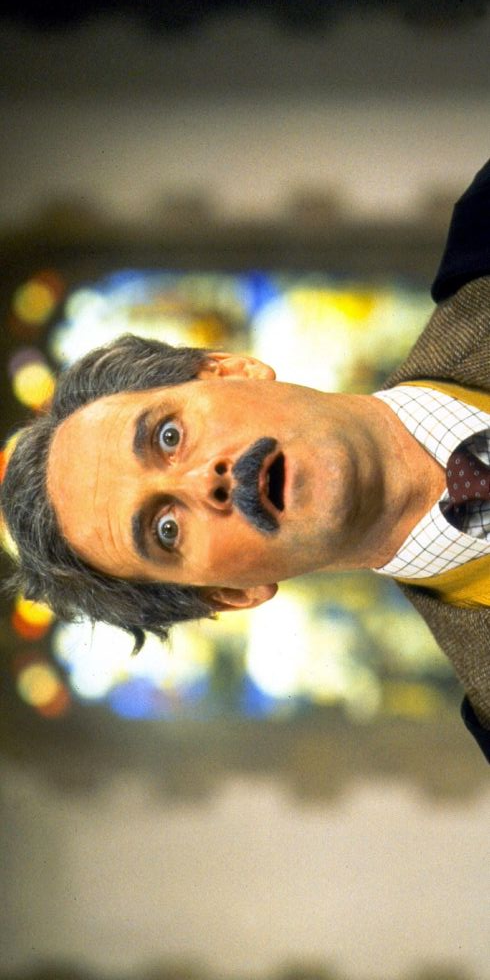
\includegraphics{media/14916935985623/rotated90.png}
\item
  Rotating \(\pi\) 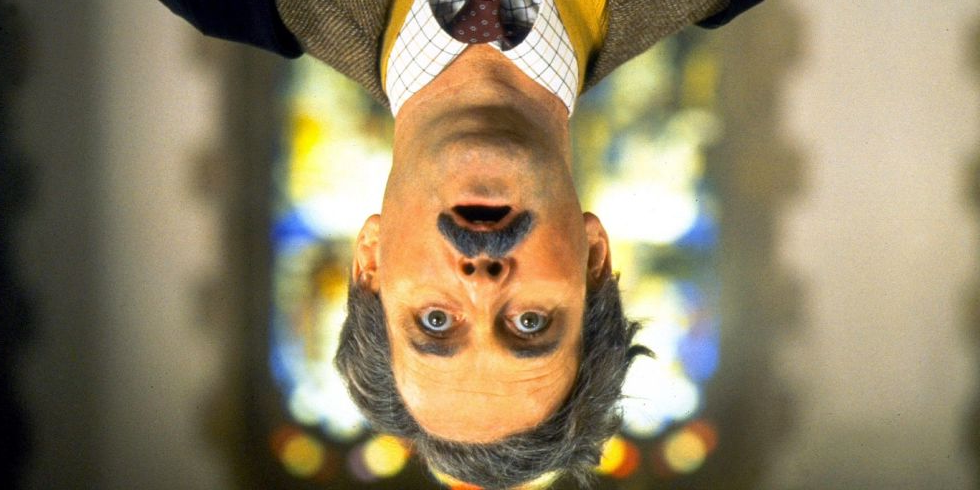
\includegraphics{media/14916935985623/rotated180.png}
\item
  Rotating \(\frac{3\pi}{2}\)
  
\includegraphics{media/14916935985623/rotated270.png}
\end{itemize}

\end{document}
